\section{Methodology}
\label{ch:method}
\noindent	

\subsection{System description}
\label{ch:method:model}
The structure of the IoT system including the planned devices can be found in figure \ref{fig:communication}. 
\begin{figure}[H]
    \centering
    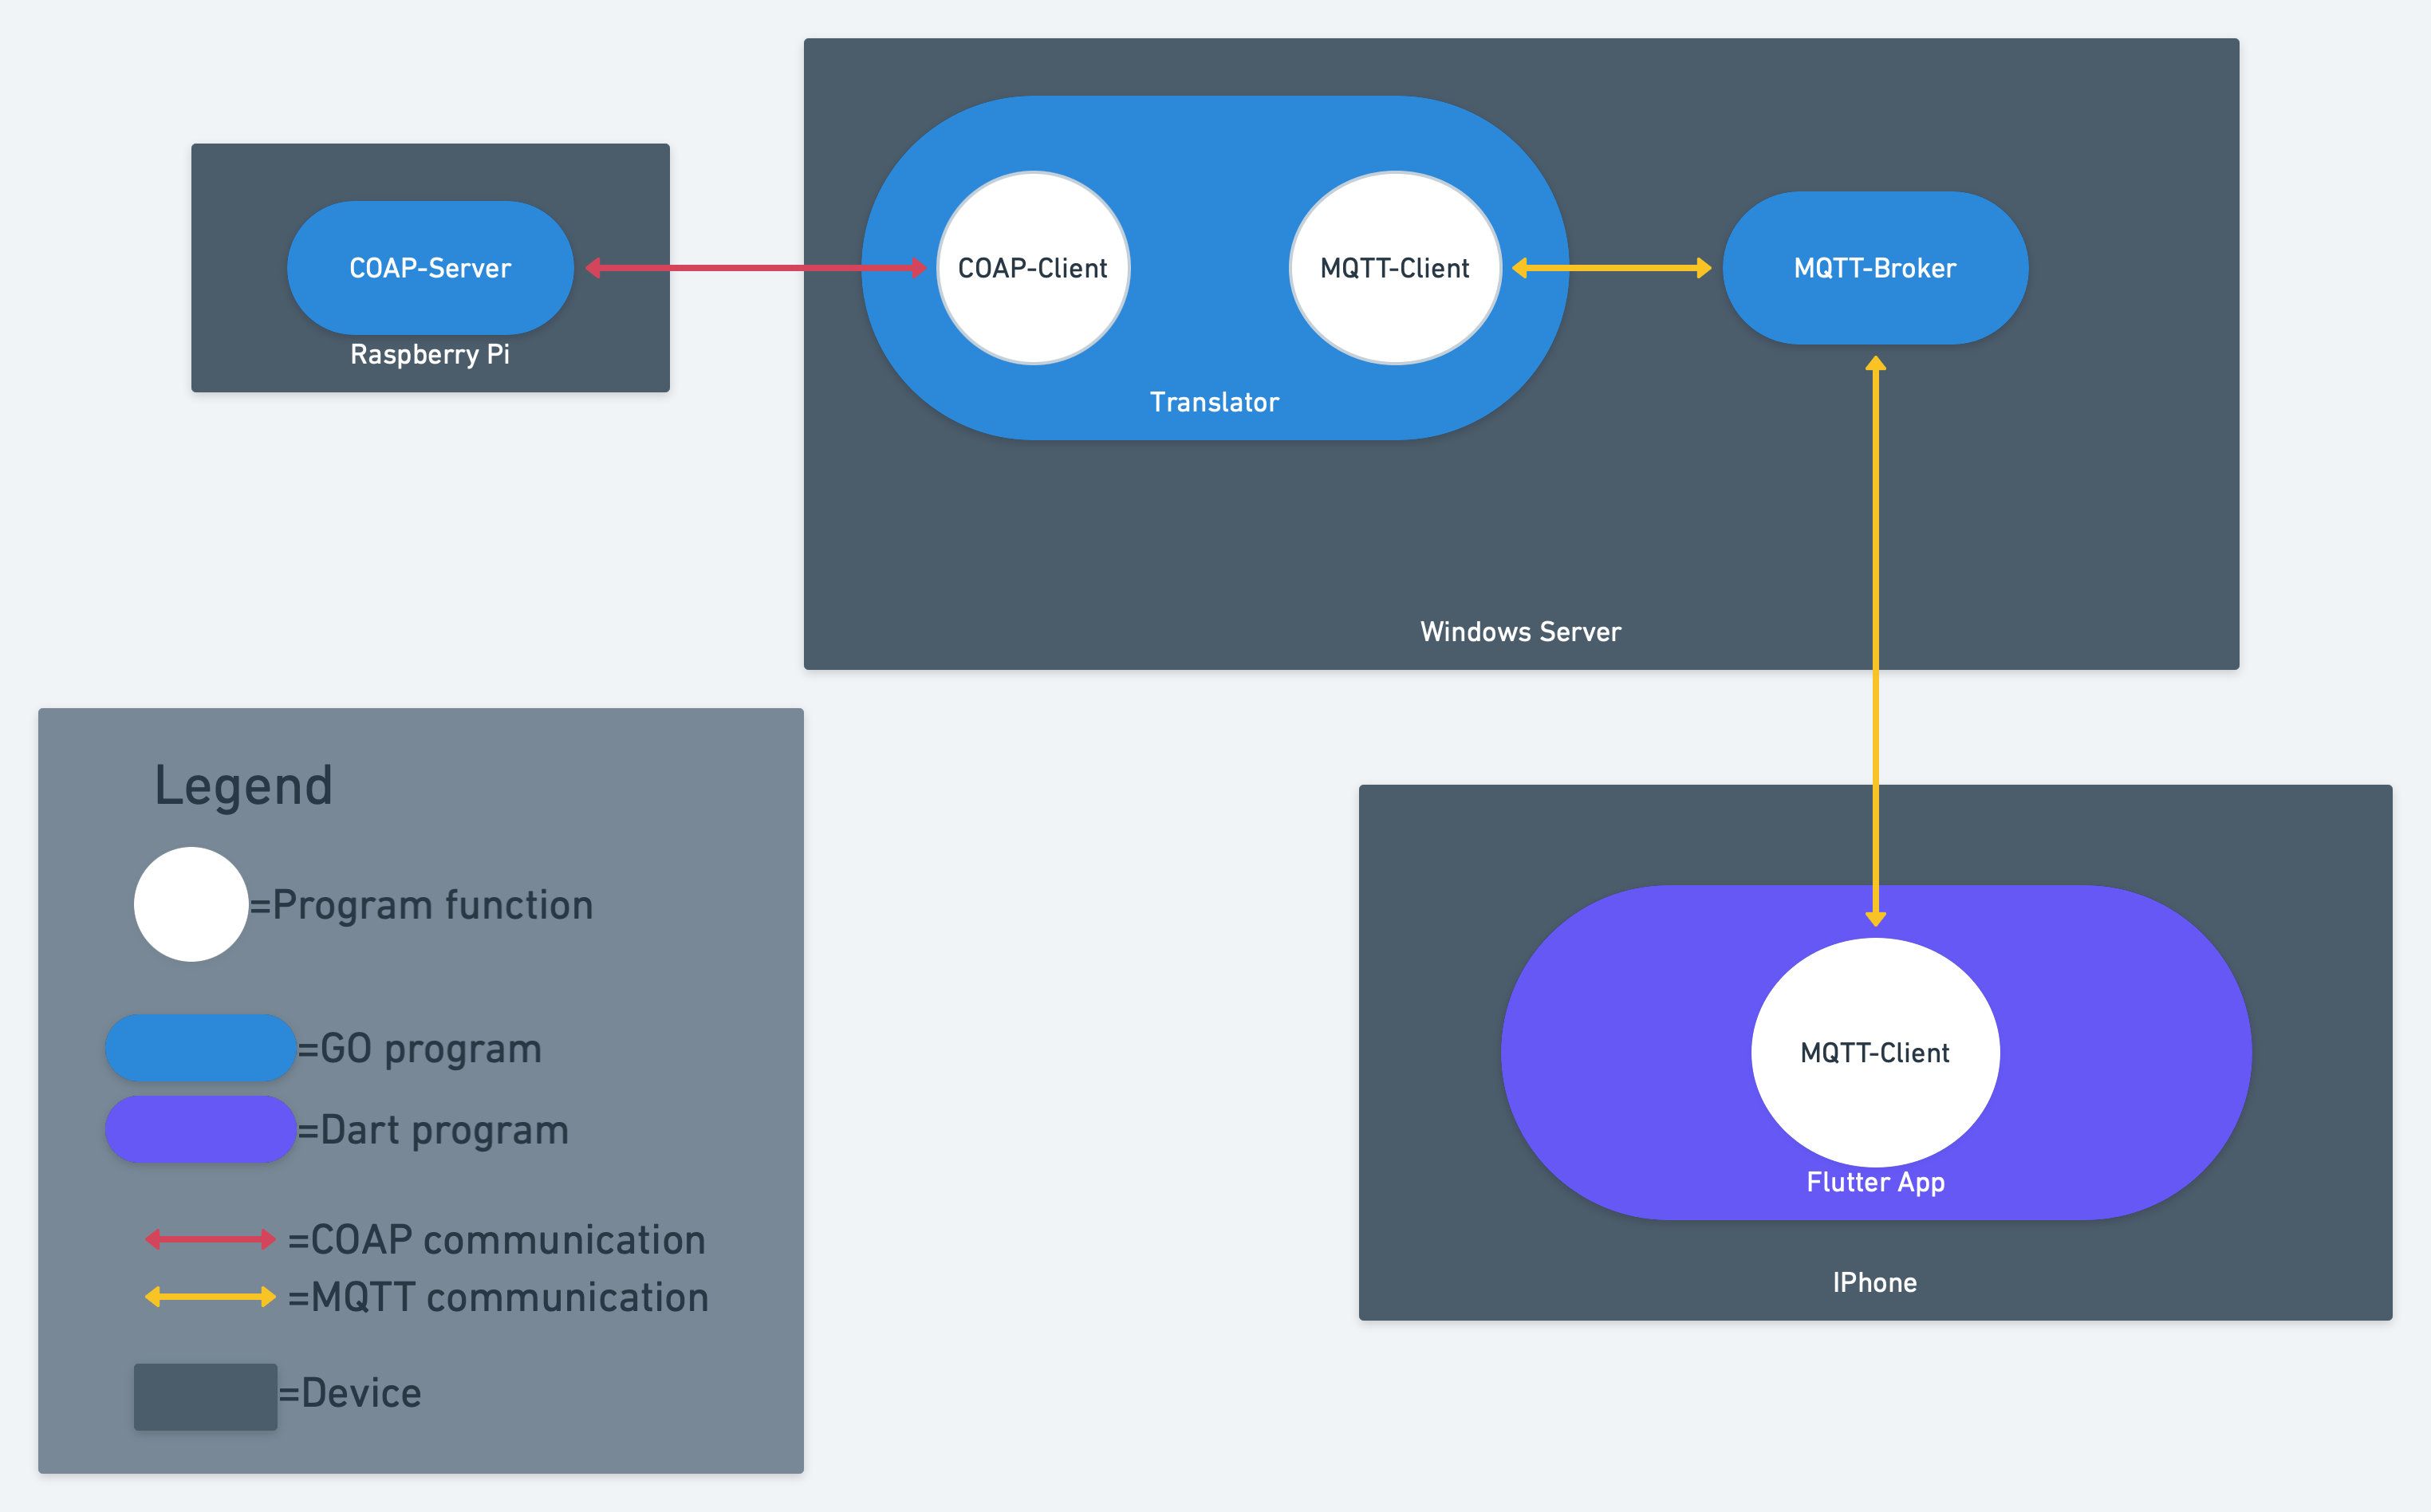
\includegraphics[width=1\textwidth]{img/communication.png} 
    \caption{The planned communication scheme. See legend for explanation}
    \label{fig:communication}
\end{figure}

The CoAP-server and the MQTT-clients will use external libraries while the MQTT-broker and the CoAP-client is implemented by me. 
The user application will be developed using Flutter and will use a Dart library written by Steve Hamblett \cite{dartMqtt}. 
All other components are written in Golang. The CoAP-server uses a library by plgd\cite{goCoAP} and the MQTT-clinet uses a library by the Eclipse Foundation \cite{goMQTT}.

The primary purpose of the server is to collect system data more specifically CPU and RAM usage. A client will then be able to request this information. Additionally, the server can create mock temperature sensors. A sensor has a location, power status and a temperature. A client can request temperature, create a sensor, change power status and remove a sensor. 

The translators have two purposes. It will collect data from the CoAP-server and publish using the MQTT-client. It will also react to published messages from other MQTT-clients and create CoAP-request accordingly. Ex. the Flutter app wants to create a sensor. The translator can then convert a publishing by the application to a CoAP POST-request.

The MQTT-broker is a standard MQTT-broker implemented using Golang. It will handle the subscription and publish messages, creating a communication channel between the translator and the Flutter application.

Lastly the Flutter application will be multi-platform application acting as the frontend of the IoT system. The app will have the following capabilities. 
\begin{itemize}
    \item Display CoAP-server system information.
    \item Display temperature sensor information.
    \item Create temperature sensors.
    \item Turn off specific temperature sensors.
    \item Delete a Temperature sensor.
    \item Run a benchmark.
    \item Display benchmark results.
\end{itemize}

The system requires one active CoAP-server, one active translator, one active MQTT broker and one or more Flutter applications. This implementation will put the CoAP-server on a Raspberry Pi running Raspbian and bundle the MQTT-broker and the Translator on a Server running Windows Server. The Flutter application will run on at least IOS but should be able to run on any operating system supported by Flutters build system.

\subsection{Evaluation}
To evaluate the system the RTT will be measured between the user Application and the CoAP server. This will be done using a benchmark function inside the Flutter application. Three benchmark runs will be done adding a new instance of the flutter application with each run to simulate different load on the system. The Flutter application will output the following metrics:
\begin{itemize}
    \item Requests per second
    \item Average RTT
    \item Max RTT
    \item Min RTT
\end{itemize}


% With regards to C- and D-level diploma work, it is insufficient to merely perform a practical construction or programming project. A systematic study must also be carried out, e.g. an evaluation and analysis of the design or program. The study should result in objective facts, preferably in the form of tables and diagrams, into which your own conclusions are built in. The study can be a verification of a design that meets the requirement specification, or a comparison of competing alternatives. It is acceptable to allow users to answer a questionnaire or be interviewed. It is also possible to evaluate web-pages and other user interfaces according to usability criteria.

% The method section is the point at which your chosen method and intended procedure during the research are discussed. This section shall not be a chronological diary filled with irrelevant details, but should contain information given in such a way that it is understandable for the reader and enables him/her to interpret your results and repeat your work, i.e. in order to check the results. Here, the tools, assumptions, mathematical models, performance measures and assessment criteria are presented. It is also at this point that the means adopted for the evaluation and verification of the computer programs and technical solution proposals are presented. This can include a test plan to check that the structure works and criteria to assess its usefulness. In research reports regarding natural science and technology this chapter is often called “Model”, “System Model” or “Simulation Model”.

% Justify your choice of methodology/model. This choice is very important, because it could be the actual key to the result of your research. Comment on the method's possible weaknesses and problems that may arise during actual implementation. Refer to the problem wording in the introduction chapter. It is possible, for example, to write “problem P1 is attempted through the method M1 and problem P2 through…” 

% In your report, you should - depending on what the report is about- find information about what you have investigated and how you have gathered and processed data. Possible questionnaires, interview questions and the likes can be presented as appendices. Detailed descriptions concerning experimental formats of possible interest to those wanting to repeat the experiment should also be included in this chapter.
